\documentclass[titlepage,11pt]{article}
\usepackage{amsmath}
\usepackage{tikz}

\begin{document}

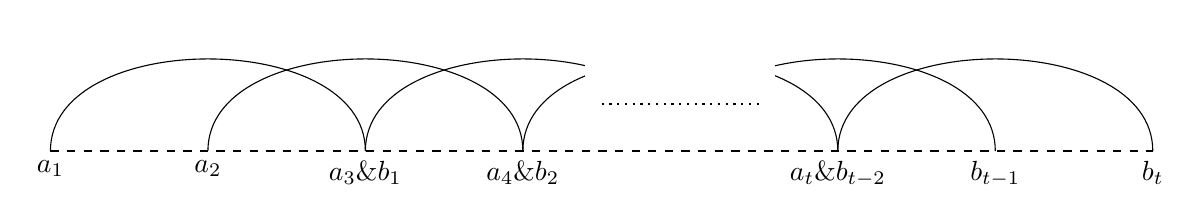
\begin{tikzpicture}[scale=1,auto=left]


\draw (0,0) to [bend left = 90] (4,0);
\draw (2,0) to [bend left = 90] (6,0);
\draw (4,0) to [bend left = 90] (8,0);
\draw (6,0) to [bend left = 90] (10,0);
\draw (8,0) to [bend left = 90] (12,0);
\draw (10,0) to [bend left = 90] (14,0);

\tikzstyle{every node}=[]
\draw[below] (0,0) node []           {$a_1$};
\draw[below] (2,0) node []           {$a_2$};
\draw[below] (4,0) node []           {$a_3\&b_1$};
\draw[below] (6,0) node []           {$a_4\&b_2$};
\draw[below] (10,0) node []           {$a_t\&b_{t-2}$};
\draw[below] (12,0) node []           {$b_{t-1}$};
\draw[below] (14,0) node []           {$b_t$};

\draw[white, fill=white] (6.8,0) rectangle (9.2,1.2);
\draw[dashed]  (0,0)--(14,0);

\draw[dotted,thick] (7,.6) -- (9,.6);
\end{tikzpicture}

\end{document}